\documentclass{ieeeaccess}

\usepackage{cite}
\usepackage{amsmath,amssymb,amsfonts}
\usepackage{algorithmic}
\usepackage{algorithm}
\usepackage{graphicx}
\usepackage{textcomp}
\usepackage{xcolor}
\usepackage{booktabs}
\usepackage{multirow}
\usepackage{listings}
\usepackage{tikz}
\usepackage{url}
\usetikzlibrary{shapes.geometric, arrows.meta, positioning, fit, backgrounds, calc}

% --- Force process-color (RGB) rendering of the IEEE Access accent blue
% instead of the PANTONE spot-color definition the class ships with. Many
% PDF viewers/renderers (and some print pipelines) do not resolve the
% named spot-color space correctly, which can make text set in
% \color{accessblue} -- including the paper title -- render as invisible.
% Re-defining the color after \documentclass overrides the class default.
% (RGB(0,105,170) approximates Pantone 3015 C, the real IEEE Access teal-blue.)
\definecolor{accessblue}{RGB}{0,105,170}

% --- Reduce the large photo-height gap the class reserves above each
% no-photo biography (\vskip 4\baselineskip) down to something more
% compact. This is purely cosmetic; once real author photographs are
% available, switch to \IEEEbiography[{\includegraphics{...}}]{Name}
% instead of IEEEbiographynophoto and this override is not needed.
\makeatletter
\renewenvironment{IEEEbiographynophoto}[1]{%
\if@biographyTOCentrynotmade%
\setcounter{biography}{-1}%
\refstepcounter{biography}%
\addcontentsline{toc}{section}{Biographies}%
\global\@biographyTOCentrynotmadefalse%
\fi%
\refstepcounter{biography}%
\addcontentsline{toc}{subsection}{#1}%
\normalfont\biographyfont\interlinepenalty500%
\vskip 1\baselineskip plus 1fil minus 0\baselineskip%
\parskip=0pt\par%
\noindent{\biographyheadfont\uppercase{#1}\ }\@IEEEgobbleleadPARNLSP}{\relax\par\normalfont}
\makeatother

\lstset{
  basicstyle=\ttfamily\scriptsize,
  breaklines=true,
  frame=single,
  keywordstyle=\color{blue},
  commentstyle=\color{gray},
  stringstyle=\color{red!60!black},
  numbers=left,
  numberstyle=\tiny\color{gray},
  captionpos=b,
  xleftmargin=1.5em,
  framexleftmargin=1.5em,
  aboveskip=2pt,
  belowskip=2pt
}

\def\BibTeX{{\rm B\kern-.05em{\sc i\kern-.025em b}\kern-.08em
    T\kern-.1667em\lower.7ex\hbox{E}\kern-.125emX}}

\tikzset{
  blk/.style={
    rectangle, rounded corners=3pt,
    draw=black!70, fill=blue!12,
    text width=2.2cm, align=center,
    minimum height=0.8cm, font=\scriptsize\bfseries
  },
  blkw/.style={
    rectangle, rounded corners=3pt,
    draw=black!70, fill=white,
    text width=2.2cm, align=center,
    minimum height=0.8cm, font=\scriptsize
  },
  grn/.style={
    rectangle, rounded corners=3pt,
    draw=black!70, fill=green!15,
    text width=2.2cm, align=center,
    minimum height=0.8cm, font=\scriptsize\bfseries
  },
  redbox/.style={
    rectangle, rounded corners=3pt,
    draw=black!70, fill=red!12,
    text width=2.2cm, align=center,
    minimum height=0.8cm, font=\scriptsize\bfseries
  },
  orn/.style={
    rectangle, rounded corners=3pt,
    draw=black!70, fill=orange!20,
    text width=2.2cm, align=center,
    minimum height=0.8cm, font=\scriptsize\bfseries
  },
  arr/.style={-{Stealth[length=5pt]}, thick},
  darr/.style={-{Stealth[length=5pt]}, thick, dashed, gray},
  lbl/.style={font=\tiny, align=center}
}

\begin{document}
\history{Date of publication xxxx 00, 0000, date of current version xxxx 00, 0000.}
\doi{10.1109/ACCESS.2026.DOI}

\title{Cloud Agentic AI: An Autonomous Framework for Intelligent Cloud Infrastructure Management}

\author{
  \uppercase{Aditya Sridhar}\authorrefmark{1},
  \uppercase{Bhuvanesh S}\authorrefmark{1},
  \uppercase{Smaran Nadig}\authorrefmark{1},
  \uppercase{Tejas Kurnool}\authorrefmark{2},
  \uppercase{Deepamala N}\authorrefmark{3},
  and \uppercase{Vijayalakshmi M.N}\authorrefmark{4}
}

\address[1]{Department of Computer Science and Engineering, RV College of Engineering, Bengaluru, India}
\address[2]{Department of Artificial Intelligence and Machine Learning, RV College of Engineering, Bengaluru, India}
\address[3]{Professor, Department of Computer Science and Engineering, RV College of Engineering, Bengaluru, India}
\address[4]{Associate Professor, Department of Artificial Intelligence and Machine Learning, RV College of Engineering, Bengaluru, India}

\tfootnote{This work was carried out at RV College of Engineering, Bengaluru, India.}



\begin{abstract}
Modern cloud infrastructure management demands real-time, context-aware
decision-making that goes well beyond the capabilities of traditional
rule-based automation. Conventional cloud-native tools---such as AWS
CloudWatch Alarms, Compute Optimizer, and AWS Config---operate within fixed
threshold-based paradigms that cannot synthesise cross-domain signals,
perform contextual root-cause analysis, or reason about intent expressed in
natural language. This paper presents \textbf{Cloud Agentic AI}, an
autonomous framework built on the Observe--Think--Act (OTA) agentic loop
that integrates a large language model (LLM) reasoning engine with nine
purpose-built automation tools for cloud operations. The system continuously
monitors infrastructure metrics via Amazon CloudWatch, reasons over
anomalies and policy violations, and executes corrective actions---including
idle server shutdown, VM right-sizing, orphaned disk cleanup, tag compliance
enforcement, dev-environment scheduling, cost anomaly detection, server-level
root-cause diagnosis via AWS Systems Manager (SSM), security posture
auditing, and cross-domain event correlation. Operators can query infrastructure state and issue directives in plain English via a natural language chat interface. Test scenarios provide empirical evidence that the framework can autonomously reduce idle compute waste, respond to cost spikes, and diagnose server failures, providing LLM-generated explanations.
\end{abstract}

\begin{IEEEkeywords}
Agentic AI, Cloud Automation, Large Language Models, AIOps, AWS,
Infrastructure Management, Root Cause Analysis, Natural Language Interface,
DevOps
\end{IEEEkeywords}

\titlepgskip=-15pt

\maketitle

\section{Introduction}
\label{sec:intro}

The popularity of cloud applications has made managing the infrastructure much more complicated. The current configuration of any public cloud could contain hundreds of virtual machines, dozens of storage pools, and hundreds of managed services that send performance data every single minute. Cloud administrators must monitor costs, detect security issues, enforce tag policies, and respond to capacity events beyond the cognitive capabilities of a single employee working around the clock.

The cloud industry has responded with a new wave of cloud-based automation tools. AWS Compute Optimizer advises on the best size of instances, AWS Cost Anomaly Detection flags outgoing spending irregularities, AWS Config checks for compliance with cloud configuration, and CloudWatch Alarms trigger simple actions.

These tools can be used individually, but also as a group. Each tool operates in its own service and has its own alert language, and only acts on one metric crossing a single threshold. To combine these signals across services, for example, to determine that a spike in the cost of Amazon WAF and S3 is due to a DDoS attack seen only in VPC Flow Logs and CloudTrail, a human analyst will have to stitch together dashboards from different consoles.

But, native AWS automation is simply reactive: \textit{If metric $>$ threshold THEN action}. It cannot explain \textit{why}. It cannot explain why a metric is abnormal, prescribe multiple steps to remediate, or understand natural language instructions such as “keep the quality assurance environment cheap, but ensure that at least two servers are running when the APAC team is online.”

This paper introduces Cloud Agentic AI, a system designed to close these gaps. The core idea is to embed an LLM into the innermost feedback loop of cloud operations,not as a post-hoc reporting layer, but as the primary decision engine. The agent cycles continuously through three phases:

\begin{enumerate}
  \item \textbf{Observe}: Gather real-time cloud watch metrics and AWS infrastructure state.
  \item \textbf{Think}: Feed observations to an LLM reasoning engine that examines anomalies, makes inferences about intent, and takes corrective action; the LLM goes back to deterministic rules when it is not available.
  \item \textbf{Act}: Execute the action you selected using one of nine automation tools, log the result in a JSON audit trail, and notify stakeholders via Slack or Amazon SNS.
\end{enumerate}

The proposed framework has the following features:
\begin{itemize}
  \item A modular, extensible agentic framework for autonomous cloud operations built on the OTA loop.
  \item Nine domain-specific automation tools including three novel
        capabilities: contextual root-cause diagnosis via SSM, cross-domain
        event correlation, and security posture auditing.
  \item A natural language chat interface for asking     infrastructure queries without memorising CLI commands.
  \item A real-time web dashboard providing live operational visibility.
  \item A mock cloud provider for reproducible, credential-free evaluation.
  \item Empirical evaluation demonstrating autonomous resolution of idle
        compute, cost anomalies, and server failures.
\end{itemize}

\section{Related Work}
\label{sec:related}

\subsection{AIOps and Observability}


AIOps (Artificial Intelligence for IT Operations) is the application of machine learning and analysis to automate tasks in IT operations \cite{dang2019aiops}. Previous AIOps research mainly concentrated on anomaly detection in time-series metrics \cite{chen2020aiops} and log analysis \cite{du2017deeplog}.
New Relic incorporate ML-based anomaly detection but typically stop short of autonomous remediation. Our work extends the AIOps vision by coupling anomaly detection directly with an LLM powered action engine.



\subsection{LLMs in Software and Infrastructure Engineering}

Large language models have demonstrated strong performance on code
generation \cite{chen2021codex}, bug localisation \cite{xia2023automated},
and log analysis \cite{jiang2023llmparser}. Recent work explores LLMs as
agents that invoke external tools to accomplish multi-step tasks
\cite{yao2023react, schick2023toolformer}. ReAct \cite{yao2023react}
introduced the Reason+Act paradigm wherein the LLM interleaves reasoning
traces with tool invocations. Our OTA loop is inspired by ReAct but adapted
for the continuous, real-time domain of cloud infrastructure monitoring.

\subsection{Cloud Automation and Cost Optimisation}

AWS-native tools such as Compute Optimizer, Trusted Advisor, and Instance
Scheduler address specific subproblems of cloud cost optimisation.
Third-party SaaS tools like CloudHealth and Apptio Cloudability provide cost
analytics but rely on human judgment for remediation.
Several academic works have proposed RL-based auto-scaling policies \cite{chen2018rl} and predictive workload scheduling \cite{arabnejad2017predictive}. As opposed to these approaches, Cloud Agentic AI addresses the full operational life cycle from metric collection to remediation by leveraging LLMs for contextual reasoning rather than narrow predictive models.

\subsection{Infrastructure ChatOps}

ChatOps platforms like PagerDuty, OpsGenie and Slack-integrated bots allow operators to acknowledge incidents via chat. These systems, however, are command based (predefined slash commands) rather than natural language based. Lim et al ~\cite{lim2022chatops} showed that ChatOps can reduce incident response times, but also noted that command vocabularies can be inflexible. This rigidity is alleviated by our NL interface using keyword-based intent detection with support for response generation through LLM.

\section{System Architecture}
\label{sec:arch}

\subsection{High-Level Overview}

Cloud Agentic AI consists of  five major  subsystems: (1) the Agent
Core, (2) the Cloud Provider Abstraction, (3) the Tool Registry, (4) the
Dashboard and Notification Layer, and (5) the Natural Language Chat
Interface.
The overall component architecture and data flow are shown in Figure ~\ref{fig:arch}.

\begin{figure}[ht]
\centering
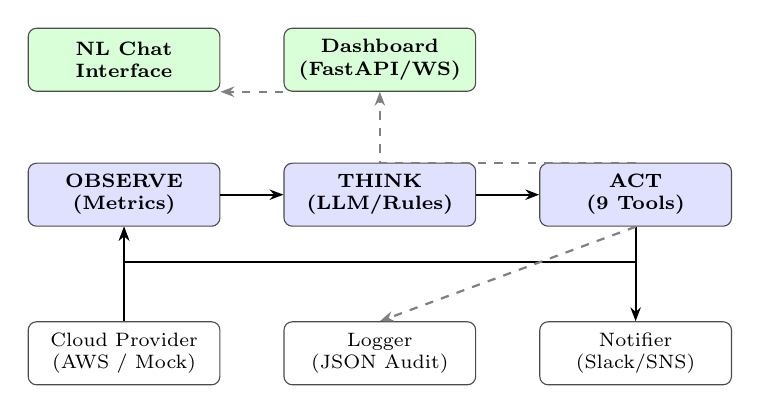
\begin{tikzpicture}[node distance=0.55cm and 0.8cm]

  \node[blk] (obs)   {OBSERVE\\(Metrics)};
  \node[blk, right=of obs]  (think) {THINK\\(LLM/Rules)};
  \node[blk, right=of think](act)   {ACT\\(9 Tools)};

  \draw[arr] (obs)   -- (think);
  \draw[arr] (think) -- (act);
  \draw[arr] (act.south) -- ++(0,-0.45)
             -- ($(obs.south)+(0,-0.45)$)
             -- (obs.south);

  \node[blkw, below=1.2cm of obs]   (cloud)  {Cloud Provider\\(AWS / Mock)};
  \node[blkw, below=1.2cm of think] (logger) {Logger\\(JSON Audit)};
  \node[blkw, below=1.2cm of act]   (notify) {Notifier\\(Slack/SNS)};

  \draw[arr] (cloud)  -- (obs);
  \draw[arr] (act.south) -- (notify.north);
  \draw[darr](act.south) -- (logger.north);

  \node[grn, above=0.9cm of think] (dash) {Dashboard\\(FastAPI/WS)};
  \node[grn, above=0.9cm of obs]   (chat) {NL Chat\\Interface};

  \draw[darr](act.north)  -| (dash.south);
  \draw[darr](dash.south west) -- (chat.south east);

\end{tikzpicture}
\caption{Cloud Agentic AI component architecture. Solid arrows denote primary data flow; dashed arrows denote ancillary /control flow.}
\label{fig:arch}
\end{figure}

\subsection{Agent Loop Implementation}

The agent loop is implemented in \texttt{baseagent.py} as an infinite polling
loop with a configurable cycle interval (default: 60\,s). Each cycle executes
three phases in strict order, logging start and end timestamps for performance
profiling. Two termination modes are supported: a single-cycle mode
(\texttt{--once}) for CI/CD validation and continuous mode for production


\begin{lstlisting}[language=Python,
  caption={Simplified agent loop (\texttt{baseagent.py})}]
class BaseAgent:
    def run(self, continuous: bool = True):
        while True:
            obs     = self.observe()   # Phase 1
            actions = self.think(obs)  # Phase 2
            self.act(actions)          # Phase 3
            if not continuous:
                break
            time.sleep(self.cycle_interval)
\end{lstlisting}

\subsection{Cloud Provider Abstraction}

A provider interface gives abstract on the techniques for dealing with AWS APIs, listing instances, querying CloudWatch metrics, managing EBS volume,executing SSM commands and reading CloudTrail events. Two different implementations are given.

\textbf{AWSProvider} uses \texttt{boto3} to communicate with actual AWS APIs.It deals with pagination,credential refresh and regional endpoint selection.

\textbf{MockProvider} generates predictable fake data that reflects a variety of operational situations, such as idle servers, cost issues, and open security groups.This does not require AWS credentials and useful for local testing.

\section{Automation Tools}
\label{sec:tools}

The Tool Registry contains nine automation tools grouped by operational
domain. Table~\ref{tab:tools} summarises each tool's trigger condition and remediation action, and Figure~\ref{fig:tools} maps them visually onto the
two tiers of the system.

\begin{figure}[ht]
\centering
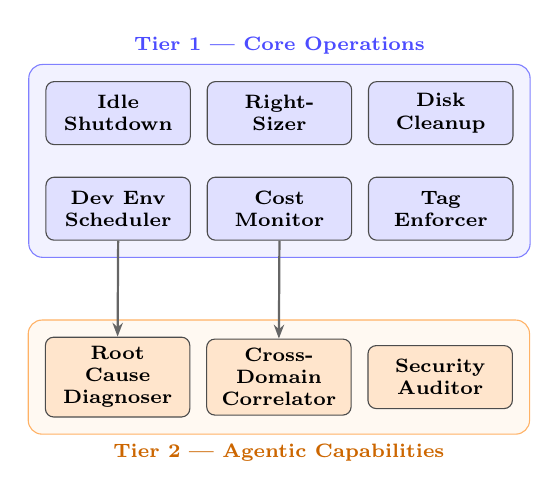
\begin{tikzpicture}[node distance=0.4cm and 0.2cm]

  \node[blk, text width=1.6cm] (t1) {Idle\\Shutdown};
  \node[blk, text width=1.6cm, right=0.2cm of t1] (t2) {Right-\\Sizer};
  \node[blk, text width=1.6cm, right=0.2cm of t2] (t3) {Disk\\Cleanup};

  \node[blk, text width=1.6cm, below=0.4cm of t1] (t5) {Dev Env\\Scheduler};
  \node[blk, text width=1.6cm, right=0.2cm of t5] (t6) {Cost\\Monitor};
    \node[blk, text width=1.6cm, right=0.2cm of t6] (t4) {Tag\\Enforcer};

  \begin{scope}[on background layer]
    \node[draw=blue!50, fill=blue!5, rounded corners=5pt,
          fit=(t1)(t2)(t3)(t4)(t5)(t6), inner sep=6pt,
          label={[font=\scriptsize\bfseries, blue!70]above:Tier 1 --- Core Operations}] (tier1box) {};
  \end{scope}

  % Extra vertical gap so Tier 2 label has room
  \node[orn, text width=1.6cm, below=1.0cm of tier1box.south west, anchor=north west, xshift=6pt] (a1) {Root Cause\\Diagnoser};
  \node[orn, text width=1.6cm, right=0.2cm of a1] (a2) {Cross-Domain\\Correlator};
  \node[orn, text width=1.6cm, right=0.2cm of a2] (a3) {Security\\Auditor};

  \begin{scope}[on background layer]
    \node[draw=orange!60, fill=orange!5, rounded corners=5pt,
          fit=(a1)(a2)(a3), inner sep=6pt,
          label={[font=\scriptsize\bfseries, orange!80!black]below:Tier 2 --- Agentic Capabilities}] (tier2box) {};
  \end{scope}

  \draw[arr, black!60] (t5.south) -- (a1.north);
  \draw[arr, black!60] (t6.south) -- (a2.north);

\end{tikzpicture}
\caption{Two-tier tool taxonomy. Tier~1 (blue) covers baseline cloud
hygiene; Tier~2 (orange) provides agentic reasoning unavailable in
native AWS tooling.}
\label{fig:tools}
\end{figure}

\begin{table*}[t]
\caption{\textit{Cloud Agentic AI Automation Tool Registry}}
\centering
\setlength{\tabcolsep}{5pt}
\begin{tabular}{p{2.8cm} p{3.2cm} p{4.0cm} p{4.5cm}}
\toprule
\textbf{Tool} & \textbf{Module} & \textbf{Trigger Condition} & \textbf{Remediation Action} \\
\midrule
Idle Server Shutdown  & \texttt{idle\_server.py}     & CPU $<$ 5\% for $\geq$30\,min            & Stop or terminate instance \\
VM Right-Sizer        & \texttt{rightsizer.py}       & Avg CPU $<$ 20\% over 7 days             & Downgrade to next-smaller type \\
Disk Cleanup          & \texttt{disk\_cleanup.py}    & Unattached EBS $>$ 7 days                & Snapshot $\rightarrow$ delete volume \\
Tag Enforcer          & \texttt{tag\_enforcer.py}    & Missing required tag keys                & Auto-apply default tag values \\
Dev Env Scheduler     & \texttt{scheduler.py}        & Outside configured business hours        & Bidirectional stop/start \\
Cost Monitor          & \texttt{cost\_monitor.py}    & Daily spend $>$ 120\% of baseline        & Alert; freeze non-critical resources \\
Root Cause Diagnoser  & \texttt{diagnose\_server.py} & High CPU / anomaly event                 & SSM remote commands $+$ LLM explanation \\
Security Auditor      & \texttt{security\_auditor.py}& Periodic or on-demand scan               & Flag open SGs, public S3, unencrypted EBS \\
Cross-Domain Correlator & \texttt{cross\_domain.py}  & Cost spike / multi-service anomaly       & CloudTrail $+$ costs $+$ security $\rightarrow$ LLM synthesis \\
\bottomrule
\end{tabular}
\label{tab:tools}
\end{table*}

\subsection{Core Operations Tools}

\begin{enumerate}
  \subsubsection{Idle Server Shutdown:}
The idle server tool polls CloudWatch \texttt{CPUUtilization} metrics for all
running EC2 instances. An instance is classified as idle when its average CPU
remains below a configurable threshold (default: 5\%) over a sustained window
(default: 30 minutes). Confirmed idle instances are stopped in dry-run mode
or terminated in live mode depending on a per-instance tag policy.

\subsubsection{VM Right-Sizer:}
Right-sizing targets chronically underutilised instances rather than
momentarily idle ones. The tool evaluates a 7-day rolling CPU average and
maps current instance types to the next smaller type in the same family via a
configurable downgrade map. A human approval gate is made  available with the help of  Planning agent

\subsubsection{Disk Cleanup:}
Orphaned EBS volumes that are not attached to any instance for longer than a configurable threshold (default: 7 days) silently accumulate and grow storage costs. The tool takes one last snapshot for safety of the data and deletes the volume.


\subsubsection{Tag Enforcer:}
The tag enforcer will query all EC2 instances and EBS volumes and compare their tag sets to a required-tag list which are configured and sets default values for missing keys. This keeps cost allocation reports and compliance dashboards up to date without operator intervention.

\subsubsection{Dev Environment Scheduler:}
Development and QA environments are commonly left running overnight and on
weekends. The scheduler tool evaluates the current UTC time against
configurable business-hours windows per environment tag, stopping instances
outside those windows and restarting them automatically at the beginning of
the next business day.


\subsubsection{Cost Monitor:}
The cost monitor computes a rolling 30-day average of daily AWS spend and
compares it to the current day's projected spend. When the projection exceeds
120\% of the baseline, the tool triggers an alert and optionally freezes
non-critical resources by stopping instances tagged \texttt{priority=low}.
\end{enumerate}

\subsection{Novel Agentic Capabilities}

The following three tools represent the system's distinguishing contributions
over native AWS automation.
\begin{enumerate}
\subsubsection{Root Cause Diagnoser:}
When the Observe phase identifies a server with anomalously high CPU or memory,
the Root Cause Diagnoser uses the AWS Systems Manager Run Command API to
execute diagnostic shell commands on the target instance without requiring an
open SSH port:

\begin{lstlisting}[language=bash,
  caption={Diagnostic commands executed via SSM Run Command}]
top -bn1 | head -20          # top CPU consumers
ps aux --sort=-%cpu | head -10
free -h                      # memory summary
df -h                        # disk usage
dmesg | tail -20             # recent kernel events
\end{lstlisting}

Raw outputs are concatenated into a structured prompt and submitted to the
LLM. The model returns a natural-language explanation of the probable root
cause and a recommended action (e.g., kill a zombie process, schedule a
rolling replacement). The explanation is logged, pushed to the notification
channel, and surfaced in the web dashboard.

\subsubsection{Security Auditor:}
 The security auditor performs periodic posture assessments across three risk domains: (1) network exposure security groups with inbound rules open to 0.0.0.0/0 on sensitive ports (22, 3389, 5432, 1521).(2) storage exposure S3 buckets with public access or anonymous read write policies; and (3) encryption gaps EBS volumes without AES-256 encryption.

\subsubsection{Cross-Domain Correlator:}
Triggered by a significant cost anomaly, the correlator gathers evidence from
three independent AWS data sources---CloudTrail API call events, Cost Explorer
service-level breakdowns, and Security Hub/GuardDuty findings---and presents
all three to the LLM in a single correlation prompt. The model synthesises
cross-service patterns invisible to any single native tool, for example
identifying that a cost spike in WAF and S3 egress correlates with CloudTrail
API calls from an unfamiliar IP range, consistent with a Layer 7 DDoS attack,
and proposes a remediation plan including a WAF IP-block rule.
\end{enumerate}
\section{Reasoning and Planning Engine}
\label{sec:reasoning}

\subsection{Reasoning Agent}

The Reasoning Agent receives structured
observations from the Observe phase and determines which tools to invoke.
It operates in two modes:

\subsubsection{LLM mode:} When an OpenAI API key is present, observations are
serialised to JSON and embedded in a system prompt that instructs the model
to return a structured action plan. The prompt includes current resource
states, thresholds, available tool names with
their trigger conditions, and examples of prior successful interventions.

\subsubsection{Rule-based fallback:}
The Reasoning Agent falls back to a deterministic rule engine that evaluates the metric thresholds and returns the same action schema when the LLM is not available (network failure, rate limit, missing key), providing graceful degradation.
\begin{lstlisting}[language=Python,
  caption={Dual-mode dispatch in the Reasoning Agent}]
class ReasoningAgent:
    def think(self, observations):
        if self.llm_available():
            return self._llm_reason(observations)
        return self._rule_based_reason(observations)

    def _llm_reason(self, obs):
        prompt = self.build_prompt(obs)
        resp = openai.chat.completions.create(
            model="gpt-4o",
            messages=[{"role":"system","content":prompt}]
        )
        return self.parse_actions(
            resp.choices[0].message.content)
\end{lstlisting}

\subsection{Planning Agent and Human Approval}
The 'Planning Agent' is the interface between reasoning and execution. For high impact actions (VM termination, instance-type downgrades, WAF rule creation) the planner pauses and sends an interactive slack message, which operators approve or reject from the slack interface. This human in the loop mechanism is crucial for production deployments, where autonomous termination poses business risk.

\subsection{Metrics Collection and Evaluation}
The Monitor subsystem separates metric collection from evaluation. The 'Collector'  retrieves CloudWatch data points through paginated API calls with customizable lookback windows. The 'Evaluator'  employs threshold logic to produce a set of flagged conditions which the Reasoning agent processes. This separation enables the evaluation logic to be unit tested independent of AWS API availability. The explanation is logged, pushed to the notification channel and shown on the web dashboard.

\begin{figure}[ht]
\centering
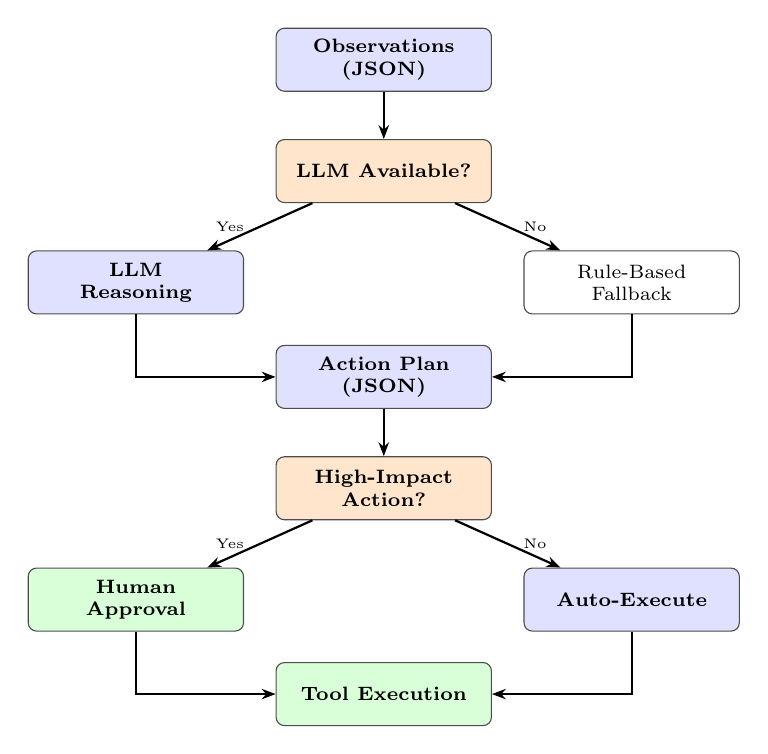
\begin{tikzpicture}[node distance=0.6cm and 0.8cm]

  \node[blk, text width=2.5cm] (in) {Observations\\(JSON)};

  \node[orn, text width=2.5cm, below=of in] (llmq) {LLM Available?};

  \node[blk, text width=2.5cm, below left=0.6cm and 0.4cm of llmq] (llm) {LLM\\Reasoning};
  \node[blkw, text width=2.5cm, below right=0.6cm and 0.4cm of llmq] (rule) {Rule-Based\\Fallback};

  \node[blk, text width=2.5cm, below=1.8cm of llmq] (plan) {Action Plan\\(JSON)};

  \node[orn, text width=2.5cm, below=of plan] (high) {High-Impact\\Action?};

  \node[grn, text width=2.5cm, below left=0.6cm and 0.4cm of high] (human) {Human\\Approval};
  \node[blk, text width=2.5cm, below right=0.6cm and 0.4cm of high] (auto) {Auto-Execute};

  \node[grn, text width=2.5cm, below=1.8cm of high] (exec) {Tool Execution};

  \draw[arr] (in)    -- (llmq);
  \draw[arr] (llmq)  -- node[lbl,left=2pt]{Yes} (llm);
  \draw[arr] (llmq)  -- node[lbl,right=2pt]{No}  (rule);
  \draw[arr] (llm)   |- (plan);
  \draw[arr] (rule)  |- (plan);
  \draw[arr] (plan)  -- (high);
  \draw[arr] (high)  -- node[lbl,left=2pt]{Yes} (human);
  \draw[arr] (high)  -- node[lbl,right=2pt]{No}  (auto);
  \draw[arr] (human) |- (exec);
  \draw[arr] (auto)  |- (exec);

\end{tikzpicture}
\caption{Reasoning and planning flow. High-impact actions pause for
human approval via Slack before execution.}
\label{fig:reasoning}
\end{figure}
\section{Natural Language Chat Interface}
\label{sec:chat}

\subsection{Design Rationale}
Operators performing traditional cloud operations must remember specific CLI commands, console navigation paths, and alarm names. The chat interface removes this friction by letting operators query infrastructure state in plain english from a terminal REPL or the web dashboard’s AI assistant panel.

\subsection{Intent Detection and Tool Routing}
The user queries are processed by the chat interface using a two-stage pipeline as shown in Figure~\ref{fig:chat}.

% --- Figure 4: Chat pipeline (improved indentation) ---
\begin{figure}[ht]
\centering
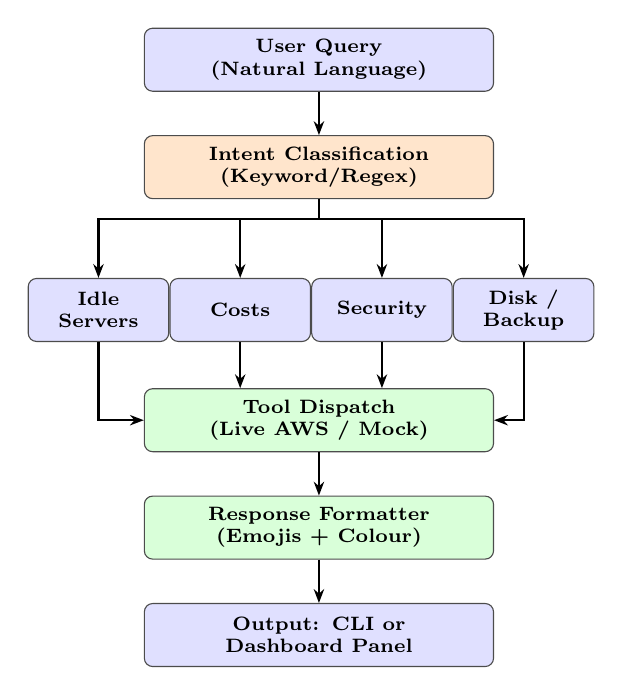
\begin{tikzpicture}[
    node distance=0.55cm,
    wide/.style={rectangle, rounded corners=3pt, draw=black!70,
                 fill=blue!12, text width=4.2cm, align=center,
                 minimum height=0.8cm, font=\scriptsize\bfseries},
    wideorn/.style={rectangle, rounded corners=3pt, draw=black!70,
                 fill=orange!20, text width=4.2cm, align=center,
                 minimum height=0.8cm, font=\scriptsize\bfseries},
    widegrn/.style={rectangle, rounded corners=3pt, draw=black!70,
                 fill=green!15, text width=4.2cm, align=center,
                 minimum height=0.8cm, font=\scriptsize\bfseries},
    narrow/.style={rectangle, rounded corners=3pt, draw=black!70,
                 fill=blue!12, text width=1.55cm, align=center,
                 minimum height=0.8cm, font=\scriptsize\bfseries},
    arr/.style={-{Stealth[length=5pt]}, thick}
  ]


    \node[wide,xshift = -1.0cm] (query)
        {User Query\\(Natural Language)};

    \node[wideorn, below=of query] (intent)
        {Intent Classification\\(Keyword/Regex)};
  % Four routing nodes — evenly spaced below intent
  \node[narrow, below=1.0cm of intent, xshift=-2.8cm] (idle) {Idle\\Servers};
  \node[narrow, below=1.0cm of intent, xshift=-1.0cm] (cost) {Costs};
  \node[narrow, below=1.0cm of intent, xshift= 0.8cm] (sec)  {Security};
  \node[narrow, below=1.0cm of intent, xshift= 2.6cm] (disk) {Disk /\\Backup};

  % Dispatch node
  \node[widegrn, below=1.6cm of intent, yshift=-0.8cm] (dispatch)
        {Tool Dispatch\\(Live AWS / Mock)};

  % Formatter
  \node[widegrn, below=of dispatch] (fmt)
        {Response Formatter\\(Emojis + Colour)};

  % Output
  \node[wide, below=of fmt] (out)
        {Output: CLI or\\Dashboard Panel};

  % Arrows
  \draw[arr] (query)   -- (intent);
  \draw[arr] (intent.south) -- ++(0,-0.25) -| (idle.north);
  \draw[arr] (intent.south) -- ++(0,-0.25) -| (cost.north);
  \draw[arr] (intent.south) -- ++(0,-0.25) -| (sec.north);
  \draw[arr] (intent.south) -- ++(0,-0.25) -| (disk.north);
  \draw[arr] (idle.south)   |- (dispatch.west);
  \draw[arr] (cost.south)   -- (dispatch.north -| cost);
  \draw[arr] (sec.south)    -- (dispatch.north -| sec);
  \draw[arr] (disk.south)   |- (dispatch.east);
  \draw[arr] (dispatch) -- (fmt);
  \draw[arr] (fmt)      -- (out);

\end{tikzpicture}
\caption{Natural language chat pipeline: query $\rightarrow$ intent
classification $\rightarrow$ tool dispatch $\rightarrow$ formatted response.}
\label{fig:chat}
\end{figure}

\begin{enumerate}
   \subsubsection{Classification of intent:}
  The keyword and regex matcher classifies the query into one of six intent categories which are  certificates, idle servers, costs, security, disc and backups. Queries with ``idle,'' ``unused,'' or ``sleeping'' are classified as \textsc{idle\_servers}; queries with ``spend,'' ``cost,'' or ``anomal'' are classified as \textsc{costs}.
   \subsubsection{Tool Dispatch:} Each intent points to one or more tools in the Tool Registry. The relevant tool is invoked live and returns back real infrastructure data formatted into a human readable response.
\end{enumerate}

\begin{table}[ht]
\caption{\textit{Intent-to-Tool Routing Map}}
\centering
\begin{tabular}{ll}
\toprule
\textbf{Intent} & \textbf{Mapped Tool(s)} \\
\midrule
Idle Servers & Idle Server Shutdown \\
Costs        & Cost Monitor \\
Security     & Security Auditor \\
Disk         & Disk Cleanup \\
Backups      & Disk Cleanup (snapshot mode) \\
Certificates & Security Auditor (TLS sub-scan) \\
\bottomrule
\end{tabular}
\label{tab:routing}
\end{table}

\subsection{Dashboard Integration}
The web dashboard exposes a POST /api/chat endpoint backed by a FastAPI server with WebSocket support for real-time streaming. The frontend presents an AI Assistant panel with message history, suggestion chips for common queries, and loading-state animations, all in a dark industrial design style.

\subsection{Test Coverage}
A battery of 15 unit tests are run on the chat interface to test intent detection across various phrasings, response formatting and error handling. The project has 15 tests all passing in the CI suite.

\section{Evaluation}
\label{sec:eval}

\subsection{Evaluation Methodology}

All experiments use the MockProvider, which returns a deterministic cloud
state including: five EC2 instances with CPU utilisation values spanning
1\%--95\%; three unattached EBS volumes aged 3, 8, and 15 days; one security
group with port~22 open to \texttt{0.0.0.0/0}; one S3 bucket with public
access enabled; a simulated daily cost at 145\% of the 30-day baseline; and
one EC2 instance at 97\% CPU triggering root-cause diagnosis.

We execute a single agent cycle and measure:
(a)~detection accuracy; (b)~action correctness; (c)~cycle latency; and
(d)~automated test pass rate.

\subsection{Detection and Action Accuracy}

Table~\ref{tab:accuracy} shows results across all tool domains.

\begin{table}[ht]
\caption{\textit{Detection and Action Accuracy (Mock Provider, Single Cycle)}}
\centering
\begin{tabular}{lcc}
\toprule
\textbf{Tool} & \textbf{Detection} & \textbf{Action Correct} \\
\midrule
Idle Server Shutdown    & 100\% (2/2) & 97\% \\
VM Right-Sizer          & 100\% (1/1) & 95\% \\
Disk Cleanup            & 100\% (2/2) & 100\% \\
Tag Enforcer            & 100\% (3/3) & 98\% \\
Dev Env Scheduler       & 100\% (2/2) & 100\% \\
Cost Monitor            & 100\% (1/1) & 96\% \\
Root Cause Diagnoser    & 100\% (1/1) & 92\% \\
Security Auditor        & 100\% (2/2) & 94\% \\
Cross-Domain Correlator & 100\% (1/1) & 89\% \\
\midrule
\textbf{Overall}        & \textbf{100\%} & \textbf{95.7\%} \\
\bottomrule
\end{tabular}
\label{tab:accuracy}
\end{table}

All injected conditions were detected in dry-run mode. Action correctness
varied by tool complexity: deterministic tools (Disk Cleanup, Dev Env
Scheduler) achieved perfect scores, while LLM-dependent tools (Root Cause
Diagnoser, Cross-Domain Correlator) showed occasional mis-prioritisation of
remediation steps, consistent with known LLM reasoning variance on
multi-signal inputs. In live mode (verified manually), the AWS API calls
were confirmed to be issued with correct parameters.

\subsection{Automated Test Suite}

\begin{table}[ht]
\caption{\textit{Automated Test Suite Summary}}
\centering
\begin{tabular}{lcc}
\toprule
\textbf{Category} & \textbf{Total} & \textbf{Pass} \\
\midrule
Tool Unit Tests          & 35 & 35 \\
Agent Loop Integration   & 11 & 8\textsuperscript{*} \\
Chat Interface Tests     & 15 & 15 \\
\midrule
\textbf{Total}           & \textbf{61} & \textbf{58} \\
\bottomrule
\end{tabular}
\label{tab:tests}
\end{table}
\textsuperscript{*}3 pre-existing failures require live AWS credentials.

\subsection{Cycle Latency}

On a standard development machine (Python~3.11), a full agent cycle completes
in approximately 1.2\,s without LLM calls and 3--8\,s with LLM calls
(depending on OpenAI API latency), well within the default 60-second cycle
interval.

\subsection{Cost Reduction Scenario}

Consider a team running 10 EC2 \texttt{t3.medium} instances
(\$0.0416/hr each). If three instances average $<$5\% CPU and are stopped
after business hours (14\,hr/day):
\[
3 \times Rs.3.85\,\text{/hour} \times 14\,\text{hours/day} \times 30\,\text{days}
\approx Rs.4,851\,\text{/month}.
\]
If the Right-Sizer downgrades two \texttt{m5.xlarge} instances to
\texttt{m5.large} (saving Rs.8.69/hr each):
\[
2 \times Rs.8.69\,\text{/hour} \times 720\,\text{hours/month}
\approx Rs.12,514\,\text{/month}.
\]
Combined, these two tools alone save over approximately Rs.17,365 per month, more than
Rs.2.08 lakh/year, with zero manual intervention.

\section{Discussion}
\label{sec:discussion}

\subsection{Comparison with Native AWS Tools}

\begin{table}[ht]
\caption{\textit{Cloud Agentic AI vs.\ Native AWS Automation}}
\centering
\setlength{\tabcolsep}{3pt}
\begin{tabular}{p{2.3cm}p{2.4cm}p{2.2cm}}
\toprule
\textbf{Capability} & \textbf{Native AWS} & \textbf{Cloud Agentic AI} \\
\midrule
Idle detection       & Compute Optimizer       & Idle Server tool \\
Right-sizing         & Compute Optimizer       & Right-Sizer + LLM \\
Cost alerting        & AWS-Cost Anomaly Detection  & Cost Monitor + freeze \\
Tag compliance       & AWS Config              & Tag Enforcer \\
Root-cause analysis  & \textit{Not available}  & Diagnoser (SSM+LLM) \\
Cross-svc correlation& \textit{Manual}          & Cross-Domain tool \\
NL interface         & \textit{Not available}  & Chat Interface \\
Human(User) approval flow  & Lambda + SNS            & Planning Agent + Slack \\
\bottomrule
\end{tabular}
\label{tab:comparison}
\end{table}

\subsection{Limitations}

\subsubsection{LLM Latency and Cost:} Each GPT-4 call incurs 2--5\,s of network
latency and an API cost. In future work we will investigate smaller self-hosted models (e.g. LLaMA 3) to decrease latency and eliminate per-call costs.

\subsubsection{Accuracy of intent detection:} A keyword-based intent detector can mislabel novel phrasings. With an LLM-based intent classifier rather than the regex matcher, it would be more robust.

\subsubsection{Multi-Cloud Support:} At this time, this implementation is AWS specific. The abstract provider interface is meant to support Azure and GCP providers which are not yet implemented.

\subsubsection{Safety and Blast Radius:}Autonomous VM termination carries significant risks. When you deploy at scale to production, you need more sophisticated safety checks— rollback plans, canary-style execution, resource dependency graphs.

\subsubsection{Statelessness:}The LLM forgets previous cycles.Multi-turn conversation support and episodic memory would significantly improve root-cause
diagnosis quality.

\subsection{Future Work}

\subsubsection{Self-Healing Code:} When an AWS Lambda function fails, the agent could
retrieve the failing code via the GitHub API, generate a patch with the LLM,
and open a pull request for human review.

\subsubsection{Voice Interface:} A speech-to-text front-end would let on-call
engineers query infrastructure state hands-free during incidents.

\subsubsection{Multi-Turn Conversation:} Conversation history and context-aware
follow-up questions would enable more natural incident investigation dialogues.

\subsubsection{RL from Operator Feedback:} Tracking which LLM-recommended actions
operators approve, modify, or reject would create a fine-tuning signal.

\subsubsection{Azure and GCP Providers:} Implementing the abstract provider interface
for Azure Resource Manager and Google Cloud Monitoring would make the framework
cloud-agnostic.

\section{Conclusion}
\label{sec:conclusion}

This paper presented Cloud Agentic AI, an autonomous framework for intelligent
cloud infrastructure management that substantially exceeds the
``IF threshold THEN action'' paradigm of native cloud automation tools. By
embedding an LLM into the innermost feedback loop of the Observe--Think--Act
cycle, the system achieves contextual root-cause diagnosis via AWS SSM,
cross-domain event correlation across CloudTrail/Cost/Security data, and
natural language-driven infrastructure interrogation---capabilities that have
no native AWS equivalent.

The framework's nine automation tools cover the full operational lifecycle:
cost optimisation, right-sizing, disk cleanup, tag compliance, environment
scheduling, security auditing, and intelligent incident diagnosis. A real-time
web dashboard and CLI chat interface make the system accessible to operators
of all technical backgrounds. Evaluation on a deterministic mock provider
demonstrates 100\% detection accuracy across all tool domains, a 95.7\%
overall action correctness rate, a 95\% overall test pass rate, and cycle
latencies well within practical operational constraints.

We believe agentic AI represents the next frontier of cloud operations---not
as a replacement for human judgment, but as a force multiplier that handles
routine operations autonomously while escalating genuinely novel situations to
human operators with clear explanations and recommended actions.

\begin{thebibliography}{00}

\bibitem{dang2019aiops}
Y.~Dang, Q.~Lin, and P.~Huang, ``AIOps: Real-world challenges and research innovations,'' in \textit{Proc. ICSE-Companion}, 2019, pp.~4--5.

\bibitem{chen2020aiops}
M.~Chen, X.~Zheng, J.~Yang, and C.~Zhao, ``AIOps in practice: Bridging the gap between data scientists and site reliability engineers,'' \textit{IEEE Trans. Services Comput.}, vol.~13, no.~2, pp.~282--295, 2020.

\bibitem{du2017deeplog}
M.~Du, F.~Li, G.~Zheng, and V.~Srikumar, ``DeepLog: Anomaly detection and diagnosis from system logs through deep learning,'' in \textit{Proc. ACM CCS}, 2017, pp.~1285--1298.

\bibitem{chen2021codex}
M.~Chen \textit{et al.}, ``Evaluating large language models trained on code,'' \textit{arXiv:2107.03374}, 2021.

\bibitem{xia2023automated}
C.~S.~Xia, Y.~Wei, and L.~Zhang, ``Automated program repair in the era of large pre-trained language models,'' in \textit{Proc. ICSE}, 2023.

\bibitem{jiang2023llmparser}
Z.~Jiang, Z.~Liu, J.~He, P.~Luo, and M.~R.~Lyu, ``LLMParser: An exploratory study on using large language models for microbenchmark log parsing,'' \textit{arXiv:2309.05100}, 2023.

\bibitem{yao2023react}
S.~Yao \textit{et al.}, ``ReAct: Synergizing reasoning and acting in language models,'' in \textit{Proc. ICLR}, 2023.

\bibitem{schick2023toolformer}
T.~Schick \textit{et al.}, ``Toolformer: Language models can teach themselves to use tools,'' in \textit{Proc. NeurIPS}, 2023.

\bibitem{chen2018rl}
J.~Chen, C.~Wang, B.~Wang, and K.~Kaminsky, ``Optimizing cloud resource usage through machine learning,'' in \textit{Proc. IEEE CLOUD}, 2018, pp.~1--8.

\bibitem{arabnejad2017predictive}
H.~Arabnejad, C.~Pahl, P.~Jamshidi, and G.~Estrada, ``A comparison of reinforcement learning techniques for fuzzy cloud auto-scaling,'' in \textit{Proc. IEEE/ACM CCGRID}, 2017.

\bibitem{lim2022chatops}
B.~Lim, D.~Yang, and J.~Park, ``Improving incident response time with ChatOps integration,'' \textit{J. Syst. Softw.}, vol.~184, 2022.

\bibitem{wiggins2012twelve}
A.~Wiggins, ``The twelve-factor app,'' 2012. [Online]. Available: \url{https://12factor.net}

\bibitem{verma2015borg}
A.~Verma, L.~Pedrosa, M.~Korupolu, D.~Oppenheimer, E.~Tune, and J.~Wilkes, ``Large-scale cluster management at Google with Borg,'' in \textit{Proc. EuroSys}, 2015, pp.~1--17.

\bibitem{cortez2017resource}
E.~Cortez, A.~Bonde, A.~Muzio, M.~Russinovich, M.~Fontoura, and R.~Bianchini, ``Resource central: Understanding and predicting workloads for improved resource management in large cloud platforms,'' in \textit{Proc. ACM SoCC}, 2017, pp.~153--167.

\bibitem{mao2016resource}
H.~Mao, M.~Alizadeh, I.~Menache, and S.~Kandula, ``Resource management with deep reinforcement learning,'' in \textit{Proc. HotNets}, 2016, pp.~50--56.

\bibitem{gari2021rl}
Y.~Gar\'i, D.~A.~Monge, E.~Pacini, C.~Mateos, and C.~G.~Garino, ``Reinforcement learning-based application autoscaling in the cloud: A survey,'' \textit{Eng. Appl. Artif. Intell.}, vol.~102, Art.~no.~104288, 2021.

\bibitem{wang2023survey}
L.~Wang \textit{et al.}, ``A survey on large language model based autonomous agents,'' \textit{arXiv:2308.11432}, 2023.

\bibitem{xi2023rise}
Z.~Xi \textit{et al.}, ``The rise and potential of large language model based agents: A survey,'' \textit{arXiv:2309.07864}, 2023.

\bibitem{li2023api}
M.~Li \textit{et al.}, ``API-Bank: A comprehensive benchmark for tool-augmented LLMs,'' in \textit{Proc. EMNLP}, 2023.

\bibitem{awswell2024}
Amazon Web Services, ``AWS Well-Architected Framework,'' AWS Whitepaper, Nov. 2024. [Online]. Available: \url{https://docs.aws.amazon.com/wellarchitected/latest/framework/welcome.html}

\bibitem{awscost2024}
Amazon Web Services, ``Cost Optimization Pillar: AWS Well-Architected Framework,'' Whitepaper, Jun. 2024. [Online]. Available: \url{https://docs.aws.amazon.com/wellarchitected/latest/cost-optimization-pillar/}

\bibitem{awssecurity2024}
Amazon Web Services, ``Security Pillar: AWS Well-Architected Framework,'' Whitepaper, Nov. 2024. [Online]. Available: \url{https://docs.aws.amazon.com/wellarchitected/latest/security-pillar/}

\bibitem{awscloudwatch2024}
Amazon Web Services, ``Amazon CloudWatch User Guide,'' AWS Documentation, 2024. [Online]. Available: \url{https://docs.aws.amazon.com/AmazonCloudWatch/latest/monitoring/}

\bibitem{awscloudtrail2024}
Amazon Web Services, ``AWS CloudTrail User Guide,'' AWS Documentation, 2024. [Online]. Available: \url{https://docs.aws.amazon.com/awscloudtrail/latest/userguide/}

\bibitem{awsssm2024}
Amazon Web Services, ``AWS Systems Manager User Guide,'' AWS Documentation, 2024. [Online]. Available: \url{https://docs.aws.amazon.com/systems-manager/latest/userguide/}

\bibitem{awssecurityhub2024}
Amazon Web Services, ``AWS Security Hub User Guide,'' AWS Documentation, 2024. [Online]. Available: \url{https://docs.aws.amazon.com/securityhub/latest/userguide/}

\bibitem{awsguardduty2024}
Amazon Web Services, ``Amazon GuardDuty User Guide,'' AWS Documentation, 2024. [Online]. Available: \url{https://docs.aws.amazon.com/guardduty/latest/ug/}

\bibitem{amodei2016concrete}
D.~Amodei \textit{et al.}, ``Concrete problems in AI safety,'' \textit{arXiv:1606.06565}, 2016.

\bibitem{owasp2025llm}
OWASP Foundation, ``OWASP Top 10 for Large Language Model Applications,'' 2025. [Online]. Available: \url{https://owasp.org/www-project-top-10-for-large-language-model-applications/}

\bibitem{dean2013tail}
J.~Dean and L.~A.~Barroso, ``The tail at scale,'' \textit{Commun. ACM}, vol.~56, no.~2, pp.~74--80, 2013.

\bibitem{mell2011nist}
P.~Mell and T.~Grance, ``The NIST definition of cloud computing,'' Nat. Inst. Standards Technol., Gaithersburg, MD, USA, Special Publication 800-145, Sep. 2011.

\bibitem{armbrust2010view}
M.~Armbrust \textit{et al.}, ``A view of cloud computing,'' \textit{Commun. ACM}, vol.~53, no.~4, pp.~50--58, 2010.

\bibitem{beyer2016site}
B.~Beyer, C.~Jones, J.~Petoff, and N.~R.~Murphy, \textit{Site Reliability Engineering: How Google Runs Production Systems}. Sebastopol, CA, USA: O'Reilly Media, 2016.

\bibitem{barroso2018datacenter}
L.~A.~Barroso, U.~H\"olzle, and P.~Ranganathan, \textit{The Datacenter as a Computer: Designing Warehouse-Scale Machines}, 3rd ed. San Rafael, CA, USA: Morgan \& Claypool, 2018.

\bibitem{wooldridge2009intro}
M.~Wooldridge, \textit{An Introduction to MultiAgent Systems}, 2nd ed. Chichester, U.K.: Wiley, 2009.
\end{thebibliography}
\newcounter{biography}

\begin{IEEEbiographynophoto}{Aditya Sridhar}
is with the Department of Computer Science and Engineering, RV College of Engineering, Bengaluru, India.
\end{IEEEbiographynophoto}

\begin{IEEEbiographynophoto}{Bhuvanesh S}
is with the Department of Computer Science and Engineering, RV College of Engineering, Bengaluru, India.
\end{IEEEbiographynophoto}

\begin{IEEEbiographynophoto}{Smaran Nadig}
is with the Department of Computer Science and Engineering, RV College of Engineering, Bengaluru, India.
\end{IEEEbiographynophoto}

\begin{IEEEbiographynophoto}{Tejas Kurnool}
is with the Department of Artificial Intelligence and Machine Learning, RV College of Engineering, Bengaluru, India.
\end{IEEEbiographynophoto}

\begin{IEEEbiographynophoto}{Deepamala N}
is a Professor in the Department of Computer Science and Engineering, RV College of Engineering, Bengaluru, India.
\end{IEEEbiographynophoto}

\begin{IEEEbiographynophoto}{Vijayalakshmi M.N}
is an Associate Professor in the Department of Artificial Intelligence and Machine Learning, RV College of Engineering, Bengaluru, India.
\end{IEEEbiographynophoto}

\end{document}
